\subsection{Bifocal distance and signal contours}
\label{sec:op5-bifocal-control-figure}

The bifocal model gives a compact example of the distinction between a
detector signal and a geometric constraint. Figure~\ref{fig:op5-geometry-controls}
compares a constant distance sum with an equal-signal contour at the same
major vertex. For a radial Yukawa kernel the ratio of the leading inward
shifts is $\mu a+2+1/(1+\mu a)$ near coincident foci, with $a$ the major
semiaxis and $\mu$ the inverse screening length. These are model curves.
They leave the physical boundary coupling and OP~5 open.

\begin{figure}[htbp]
\centering
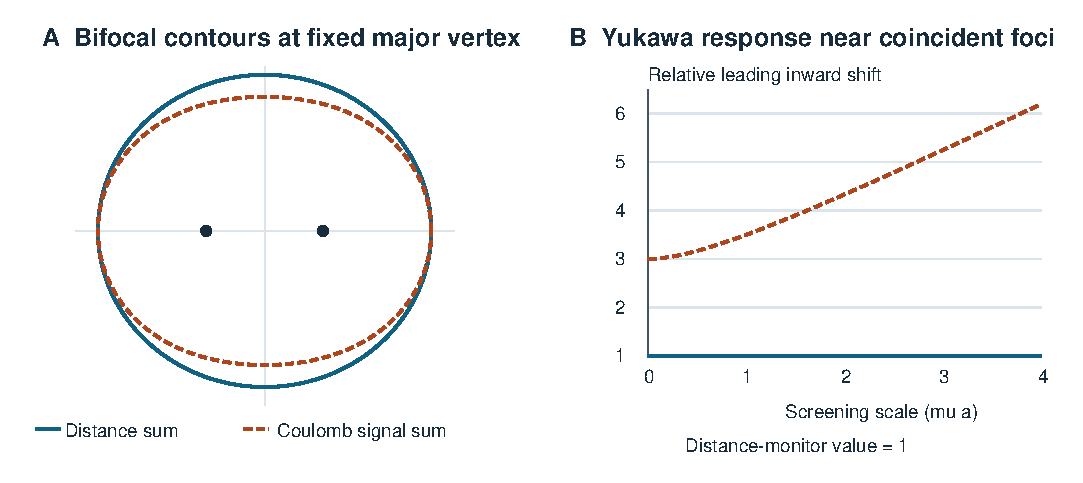
\includegraphics[width=\linewidth]{figures/op5_geometry_controls.pdf}
\caption{Bifocal geometry and signal response. Left: distance and Coulomb
signal contours at fixed major vertex, with half-separation $w/a=0.35$.
Dots mark the foci. Right: the leading inward shift for a Yukawa signal
relative to the distance-monitor shift as $\mu a$ varies.}
\label{fig:op5-geometry-controls}
\end{figure}
